\subsection{Übersichtsseite}
\setauthor{Zoe Emily Öllinger}

\subsubsection{Tabellenansicht}
\setauthor{Zoe Emily Öllinger}

Zu Beginn wurde die Tabelle erstellt auf der Übersichtsseite, hier werden die wichtigsten Daten der Kunden, für die Mitarbeiter dargestellt.
Man muss beachten, dass das Design der finalen Version des Dashboards von der Figma Version abweicht, da die Firma intern Code guidelines hat, an die wir uns halten mussten.
Ebenfalls gab es styling Guidelines und Komponenten die uns zu Verfügung gestellt wurden, wie zum Beispiel die Pagination.

\begin{figure}[h]
    \centering
    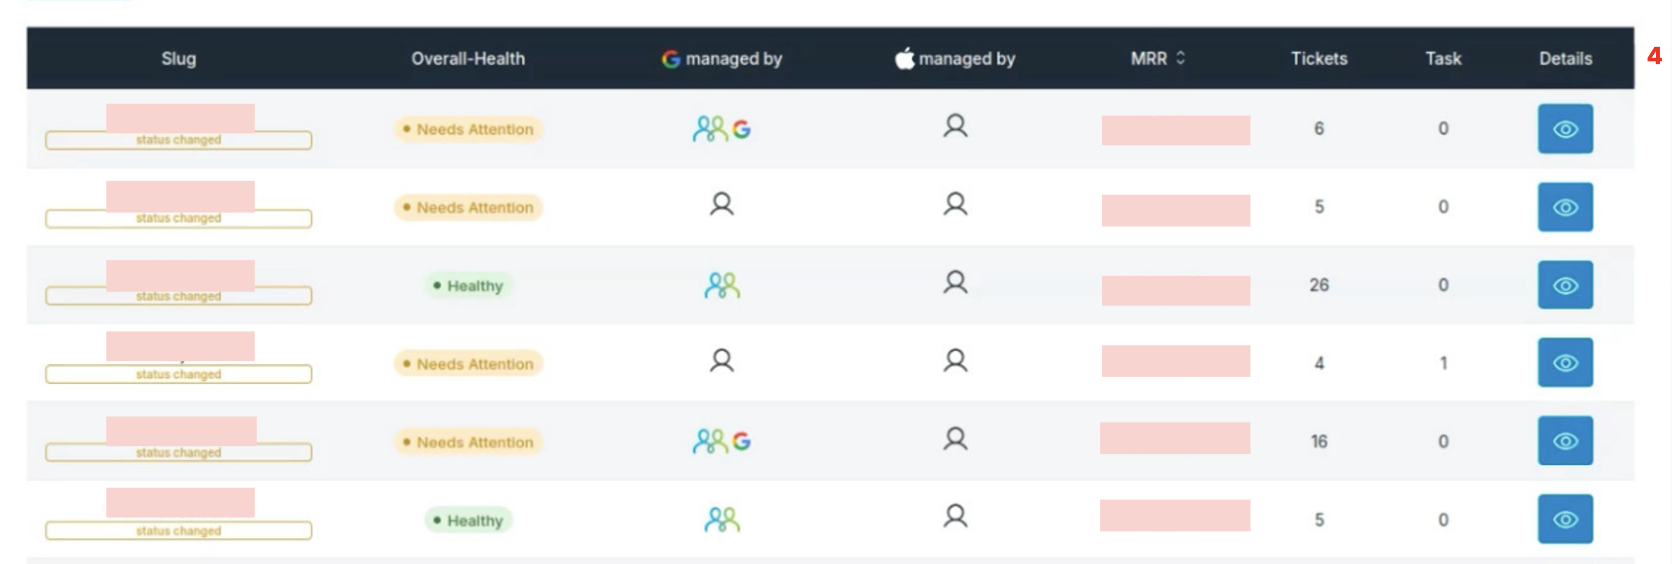
\includegraphics[width=0.8\textwidth]{pics/P4}
    \label{fig:Dashboard-Tabelle}
    \caption{Dashboard-Tabelle}
\end{figure}

Hier werden angezeigt:
\begin{compactitem}
\item der Slug (Eindeutiger Kundenbezeichner; zeigt auch ein status changed-Tag, falls sich der Status geändert hat)
\item Overall-Health (Ampelstatus des Clients (Healthy, Needs Attention, Unhealthy, Critical))
\item Google managed by (Zuständiges Team/Person für den Google-Account)
\item Apple managed by (Zuständiges Team/Person für den Apple-Kanal)
\item MRR (Monthly Recurring Revenue)
\item Tickets (Anzahl offener Support-Tickets)
\item Task (Anzahl offener Aufgaben)
\item Details (Link zur Detailseite)
\end{compactitem}

Da die Tabelle das Herzstück des Dashboards ist wurde sie als erstes implementiert und alles andere darauf aufgebaut.
Bei der Tabelle wurde auch daraus geachtet, dass die Columns filterbar sind nach dem höchsten oder niedrigsten MRR.

\subsubsection{Suchfunktion}
\setauthor{Zoe Emily Öllinger}

\begin{figure}[h]
    \centering
    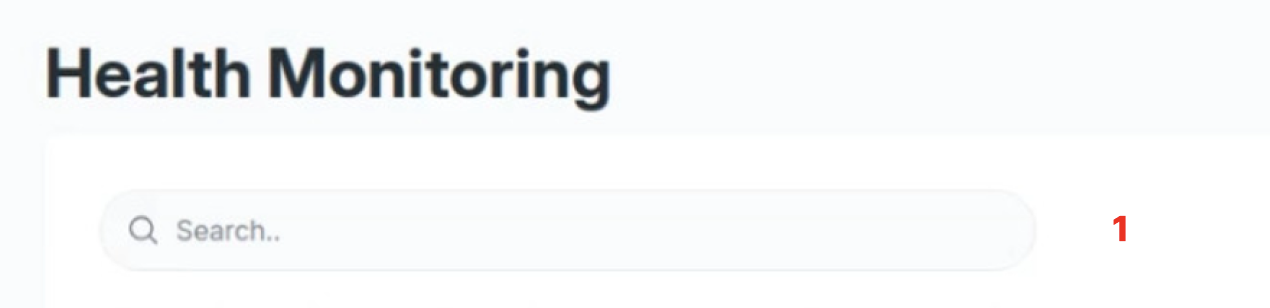
\includegraphics[width=0.8\textwidth]{pics/P1}
    \label{fig:Suchfunktion}
    \caption{Suchfunktion}
\end{figure}

Als nächstes wurde eine Suchfunktion implementiert, bei der man nach dem Slug filtern kann.
Die Suchfunktion ist hierbei caseinsensitive.

\subsubsection{Quickfilter}
\setauthor{Zoe Emily Öllinger}

\begin{figure}[h]
    \centering
    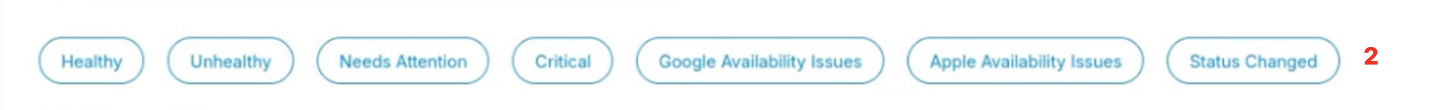
\includegraphics[width=0.8\textwidth]{pics/P2}
    \label{fig:Quickfilter}
    \caption{Quickfilter}
\end{figure}

Um den Mitarbeitern eine möglichst schnelle Filteroption zu bieten, gibt es die Quickfilter, diese sind als multiselect implementiert worden.
Das heißt man kann zum Beispiel nach allen Apps filtern, die unhealthy sind und mit status changed geflagged sind.
Das bedeutet, die App war gestern noch auf Healthy oder Needs Attention und ist heute aus den Stores geflogen.

Was bedeuten die Quickfilter Optionen?
\begin{compactitem}
    \item Healthy (Die App weist keine Fehler auf)
    \item Needs Attention (Die App wird bald aus den Stores entfernt)
    \item Critical (Die App wurde aus den Stores entfernt und ist nichtmehr verfügbar)
    \item Unhealthy (Der Status der App ist entweder Needs Attention oder Critical. Hier muss etwas getan werden!)
    \item Google Availability Issues (Der Google Playstore weist Probleme bei der App auf)
    \item Apple Availability Issues (Der Appstore weist Probleme bei der App auf)
    \item Status Changed (Der Status hat sich zum Vortag verändert)
\end{compactitem}

Das Filtern wird hier vom Frontend übernommen, da wir alle Daten der Tabelle benötigen und diese schon in das Frontend geladen haben.
Würden wir wieder eine Request an das Backend schicken, würden wir unnötig Zeit des Benutzers verschwenden.

\subsubsection{Advanced Filter}
\setauthor{Zoe Emily Öllinger}

\begin{figure}[h]
    \centering
    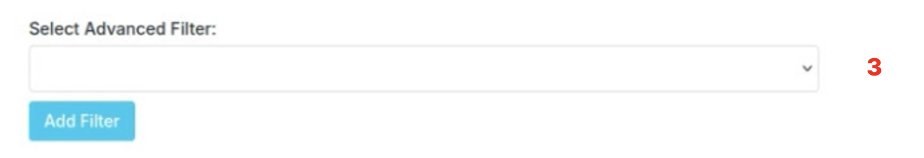
\includegraphics[width=0.8\textwidth]{pics/P3}
    \label{fig:AdvancedFilter}
    \caption{AdvancedFilter}
\end{figure}

Die Advanced Filter wurden erst zum Schluss implementiert, da diese Filteroption durch das Backend passiert.
Wir bekommen alle vorhandenen Fehler die vorkommen vom Backend ins Frontend und diese werden als zweiteilige Filteroption dargestellt.
Zuerst wählt man aus nach was man Filtern möchte zum Beispiel Google Availability und danach muss man auswählen welchen spezifischen Error Code man ansehen möchte.
Hier auch wieder ein Beispiel man hat Google Availability ausgewählt mit dem spezifischen Error Code License Agreement ran out.
Das Frontend hat keinen Zugriff auf die Error Codes der einzelenen Apps, daher wird eine Anfrage an das Backend geschickt mit dem Error Code nachdem gefiltert werden soll.
Anschließend wird die Liste neu gefiltert.
Da wir eine sehr große menge an Daten durchgehen müssen, dauert dieser Vorgang auch dementsprechend lange.

\subsubsection{Finale Version der Übersichtsseite}
\begin{figure}[h]
    \centering
    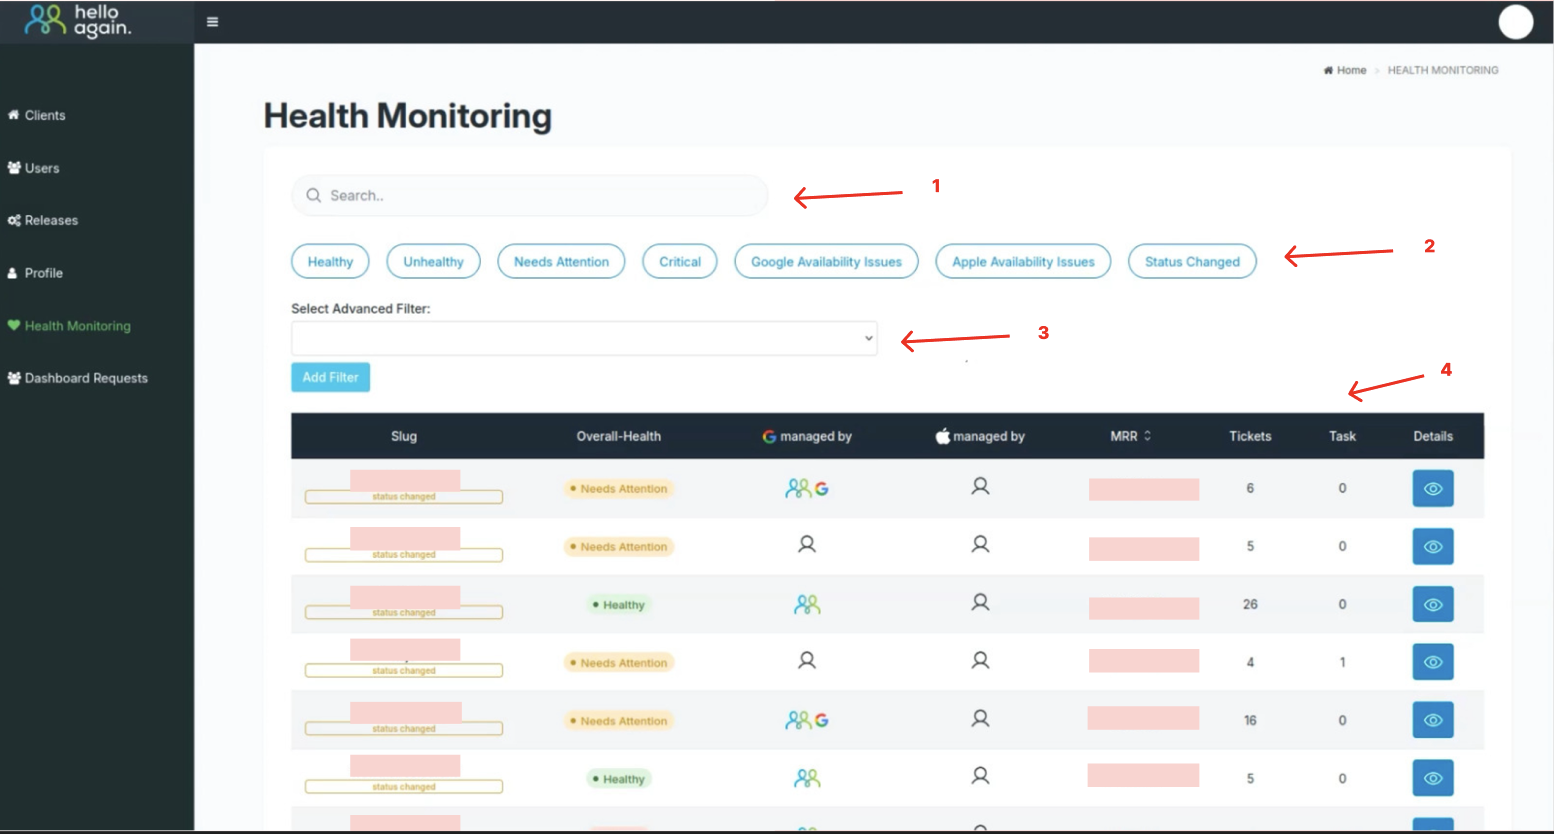
\includegraphics[width=0.8\textwidth]{pics/P5}
    \label{fig:Uebersichtsseite}
    \caption{Übersichtsseite}
\end{figure}
\clearpage
\subsection{Detailseite}
\setauthor{Zoe Emily Öllinger}

\subsubsection{Status Changed}
\setauthor{Zoe Emily Öllinger}

\begin{figure}[h]
    \centering
    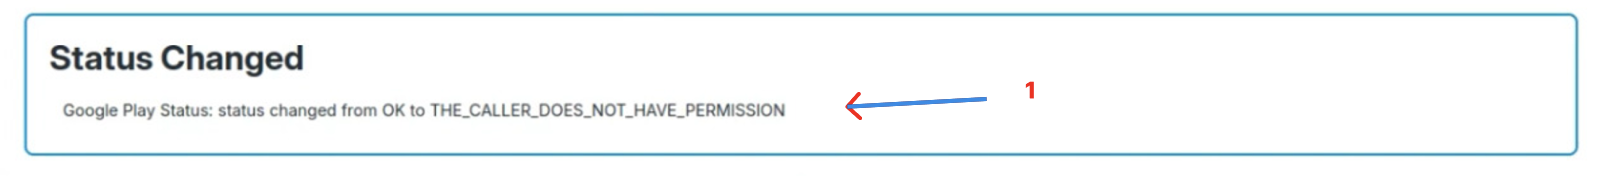
\includegraphics[width=0.8\textwidth]{pics/P8}
    \label{fig:StatusChanged}
    \caption{Status Changed}
\end{figure}

Am Anfang der Detailseite befindet sich die Status-Changed Flag.
Dieser wird nochmal visuell hervorgehoben und zeigt an wie sich die App im gegensatz zum Vortag verändert hat.
Sollte die App den Status von Healthy zu Unhealthy verändern wird der Error Code, der für diesen Fehler verantwortlich ist auch angezeigt.
Somit weiß der Benutzer sofort wo das Problem liegt.
Status Changed wird allerdings auch angezeigt, wenn die App sich von Unhealthy zu Healthy ändert, so können die Mitarbeiter zum Beispiel nach der App, die gestern noch Fehlerhaft war suchen und sehen auf den ersten Blick, ob sich ihr Status verändert hat.
Die Status changed Flags werden hier über eine Fetch-Request ins Frontend geladen.

\subsubsection{General Data}
\setauthor{Zoe Emily Öllinger}

\begin{figure}[h]
    \centering
    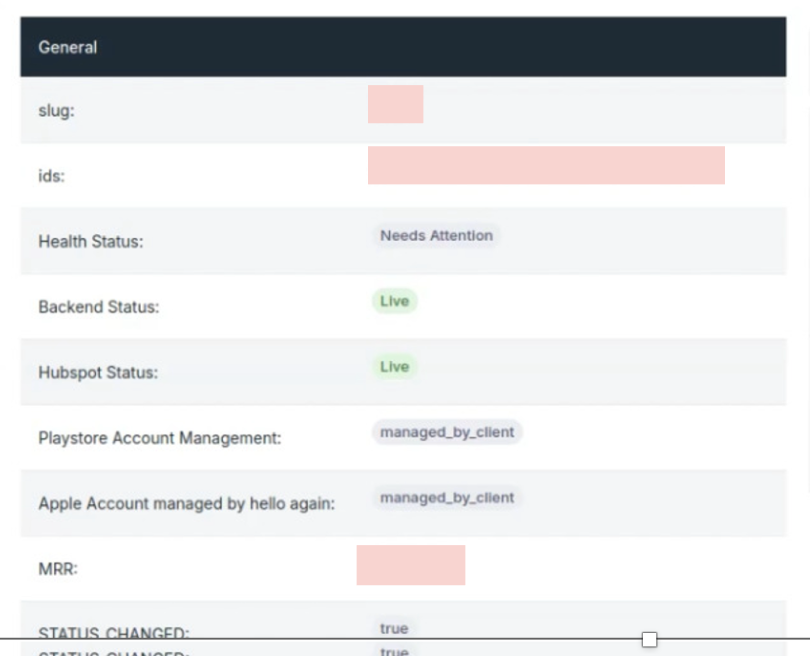
\includegraphics[width=0.8\textwidth]{pics/P9}
    \label{fig:GeneralData}
    \caption{General Data}
\end{figure}

Unter dem Status Changed Flag werden nochmals generelle Daten der App angezeigt, die auf der Übersichtsseite schon einsehbar sind.
Hier wurde darauf geachtet, dass die Daten jederzeit erweiterbar sind.
Das heißt, wenn wir aus dem Backend ergänzend noch YRR Daten bekommen würden, würde das Frontend sie ohne fremdeinwirkung eines Entwicklers darstellen.

\subsubsection{Kommentar Sektion}
\setauthor{Zoe Emily Öllinger}

\begin{figure}[h]
    \centering
    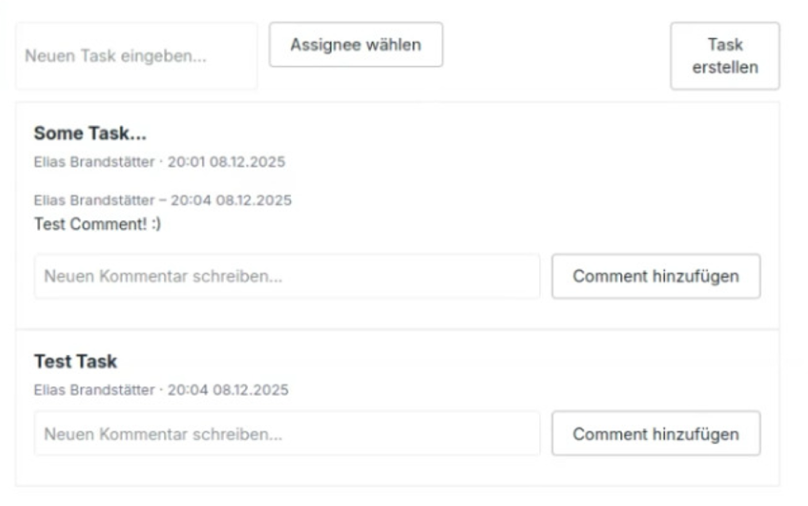
\includegraphics[width=0.8\textwidth]{pics/P10}
    \label{fig:KommentarSektion}
    \caption{Kommentarsektion}
\end{figure}

Die Kommentarsektion ist eine der wichtigsten Funktionen der Detailsseite.
Hier können Kommentare und Tasks erstellt werden, die ebenso in Asana erstellt werden.
Ebenso werden die Kommentare und Tasks, die bereits in Asana vorhanden sind dargstellt.
Wenn man einen Task erstellt kann man auch noch einen Assignee wählen, dem dieser Task dann zugeteilt wird.
Hierzu bekommen wir aus dem Backend alle Namen der Mitarbeiter, die auf dieses Asana Board Zugriff haben.
Wenn wir einen Task erstellen, wird der Text, der Slug und der Name des Assignees an das Backend übergeben, dass dan anschließend den Task in Asana erstellt.

\subsubsection{Health-Checks}
\setauthor{Zoe Emily Öllinger}

\begin{figure}[h]
    \centering
    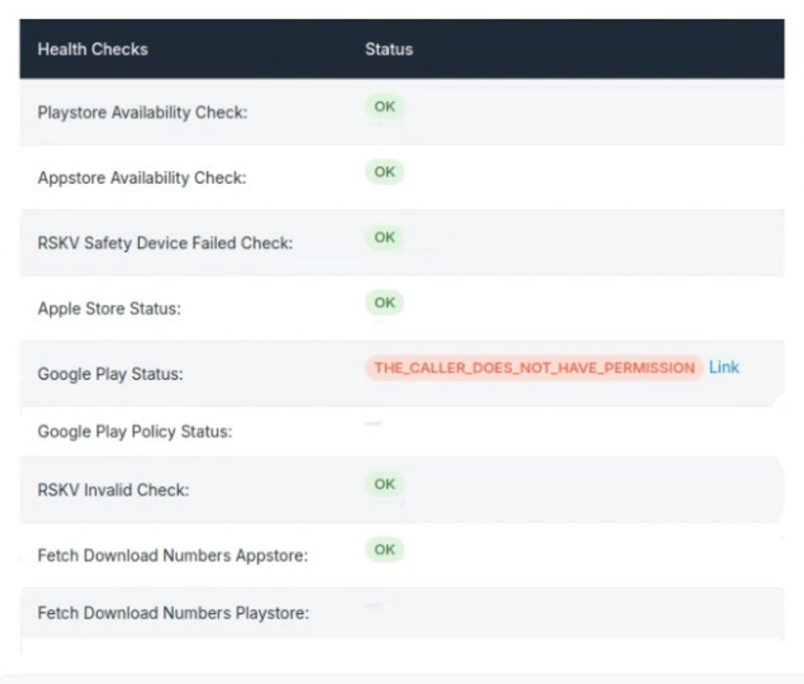
\includegraphics[width=0.8\textwidth]{pics/P11}
    \label{fig:Health-Checks}
    \caption{Health-Checks}
\end{figure}
\clearpage

Eine weitere wichtige Funktion der Detailseite sind die Health-Checks.
Hier wird der Status farblich gekennzeichnet, dass man sofort erkennt welche App Probleme wirft.
Wenn ein Error vorliegt wird immer dessen Fehlermeldung angezeigt, sowie ein Link zu Fehlerbehebung.
Drückt man auf den link wird man zur passenden Fehlerbeheungsdokumentation oder Anleitung in Confluence weitergeleitet.
Diese Health-Checks sowie die passenden Links der Doku werden vom Backend bereitgestellt.


\subsubsection{Tasks und Tickets}
\setauthor{Zoe Emily Öllinger}

\begin{figure}[h]
    \centering
    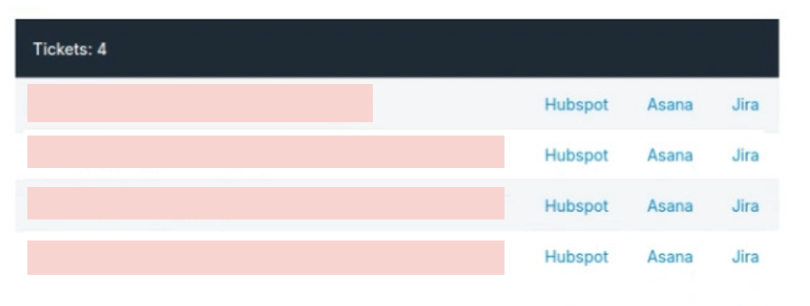
\includegraphics[width=0.8\textwidth]{pics/P12}
    \label{fig:TasksundTickets}
    \caption{Tasks und Tickets}
\end{figure}

Es wurde außerdem gewünscht, dass die Tasks und Tickets dargestellt werden, da alle 3 miteinander intern verlinkt sind.
Daher wird der Text beziehungsweise die Beschreibung der jeweils offenen Tickets angezeigt und die Links zur jeweiligen Plattform.
Wichtig ist zu betonen, dass hier nur offenene Tickets dargestellt werden.

\subsubsection{Finale Version der Detailsseite}
\setauthor{Zoe Emily Öllinger}

\begin{figure}[h]
    \centering
    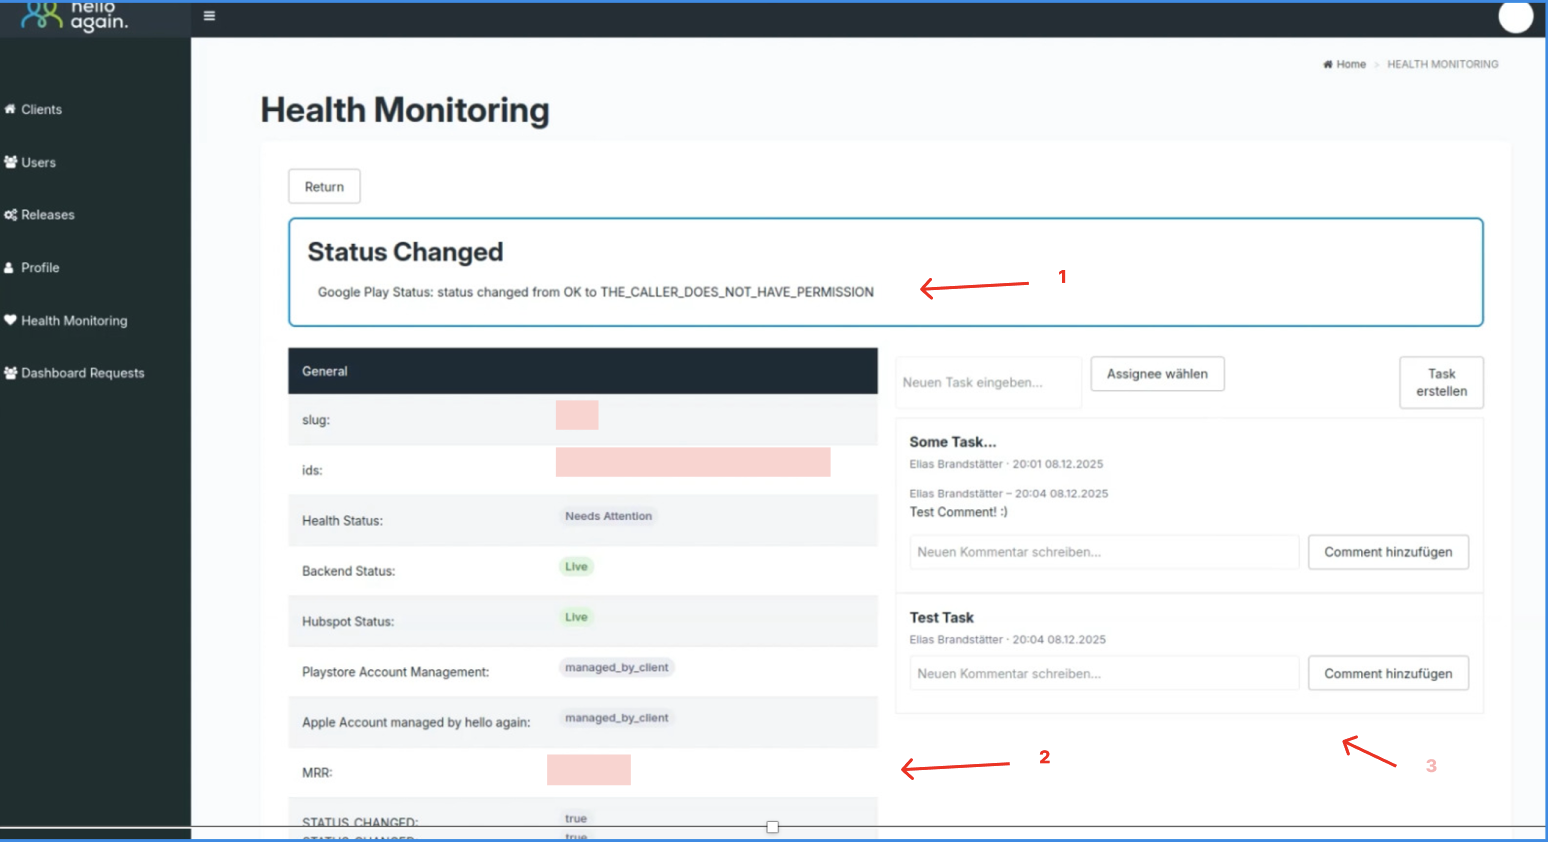
\includegraphics[width=0.8\textwidth]{pics/P6}
    \label{fig:FinaleVersionDetailseite1}
    \caption{Finale Version Detailseite 1}
\end{figure}

\begin{figure}[h]
    \centering
    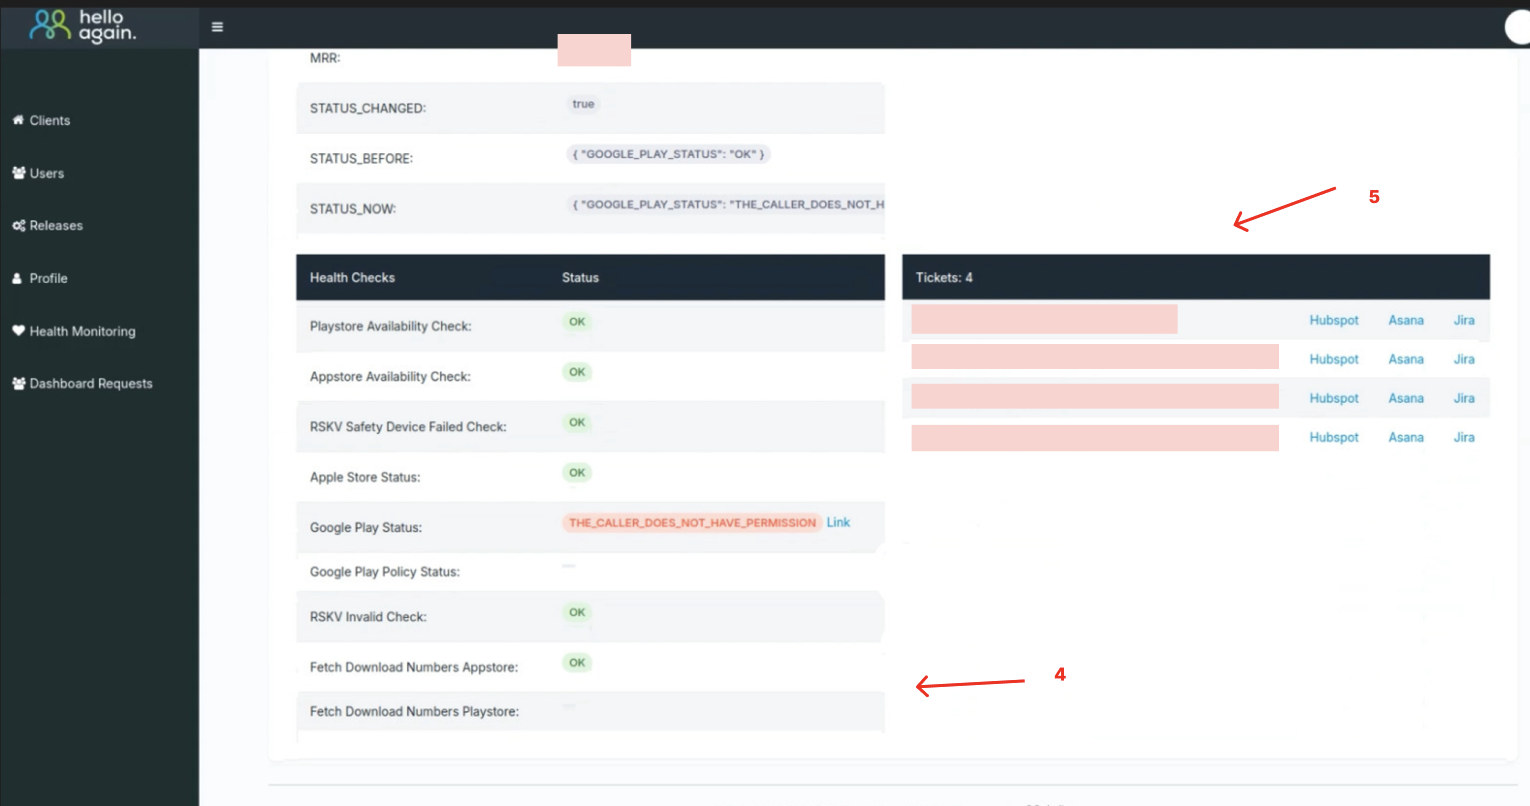
\includegraphics[width=0.8\textwidth]{pics/P7}
    \label{fig:FinaleVersionDetailseite2}
    \caption{Finale Version Detailseite 2}
\end{figure}
